\documentclass[a4paper]{article}
% Margins
\usepackage{a4wide}
% Write dutch
\usepackage[dutch]{babel}
% Used for images
\usepackage{graphicx}
% Needed to use headers
\usepackage{fancyhdr}
% Used for the euro symbol
\usepackage[gen]{eurosym}
% Used for optimal usage of gensymb
\usepackage{textcomp}
% Used for the degree symbol
\usepackage{gensymb}
% Used for captions and subcaptions on images
\usepackage{caption}
\usepackage{subcaption}
% Used for tables
\usepackage{tabu}
% Used for colors
\usepackage{xcolor}
% No tab at start of paragraph
\setlength{\parindent}{0em}
\setlength{\parskip}{1em}
% Allows to change margin for a block
\def\changemargin#1#2{\list{}{\rightmargin#2\leftmargin#1}\item[]}
\let\endchangemargin=\endlist 
% Header
\pagestyle{fancy}
\fancyhf{}
\renewcommand{\headrulewidth}{0pt}
\fancyhead[HR]{\thepage}
\fancyhead[L]{Titouan Vervack}
\begin{document}
\begin{titlepage}
\fontsize{12pt}{14pt}\selectfont

\begin{center}

% Het logo van de Universiteit Gent

\includegraphics[height=3cm]{ruglogo}

\vspace{1cm}

\fontsize{14pt}{17pt}\selectfont
% De Faculteit:
\textsc{Faculteit Wetenschappen}
\fontsize{12pt}{14pt}\selectfont
\vspace{0.3cm}

\vspace{1.2cm}

Academiejaar 2014--2015

\vspace{2.8cm}

\fontsize{17.28pt}{21pt}\selectfont

% De titel van de thesis:
\textsc{Project Datastructuren en Algoritmen III}
\fontsize{14.28pt}{21pt}\selectfont
\textsc{Gedistribueerde Genetische Algoritmen}

\fontseries{m}
\fontsize{12pt}{14pt}\selectfont

\vspace{2.8cm}

% De auteur van de thesis:
Titouan Vervack

\end{center}
\end{titlepage}
\newpage
\fontsize{12pt}{16pt}\selectfont

\section{Gemaakte beslissingen}
\subsection{Hoe controleer je of een punt binnen de veelhoek ligt}
Om te testen of een punt in de veelhoek ligt kijk ik eerst of de veelhoek niet boven of onder het punt ligt, indien dit zo is weet ik al dat het punt er zeker niet in ligt.
Het algoritme zelf zal de veelhoek opsplitsen in twee lijnen. Deze lijnen verkrijgen we door de veelhoek door te knippen aan het punt met de grootste en het punt met de kleinste y-waarde. Dan kijken we of het punt links van de rechterlijn ligt en rechts van de linkerlijn ligt. Indien beiden waar zijn ligt het punt in de veelhoek.
\subsection{Hoe stel je een organisme voor}
Een organisme wordt voorgesteld als een verzameling van punten. Deze verzameling is even groot als het aantal te plaatsen punten.
\subsection{Hoe werkt crossover}
Voor crossover sorteren we eerst onze populatie volgens fitness. Dan gaan we willekeurig twee verschillende ouders kiezen om een kind te maken. Dit is echter niet volledig willekeurig, elementen met een grote fitness hebben twee keer zoveel kans om gekozen te worden dan elementen met een kleine fitness. Het nieuwe kind wordt gevormd door de eerste helft van zijn punten te kopieren van de vader en de tweede helft van de moeder. Organismen in de populatie kunnen ook slechts \'e\'en maal per iteratie ouder zijn van een organisme, dit zorgt voor een grotere hoeveelheid variatie dan met niet unieke ouders. Het aantal kinderen is een fractie van de populatiegrootte.
\subsection{Hoe werkt mutatie}
Elk nieuw organisme dat is verwekt in de crossover heeft een kans op een mutatie. Indien hij moet muteren wordt een willekeurig punt uit het organisme geselecteerd. Dan worden er twee kleine willekeurige getallen gegenereerd, \'e\'en wordt opgeteld bij of afgetrokken van de x-waarde de andere wordt opgeteld bij of afgetrokken van de y-waarde van het punt. Deze willekeurige getallen liggen tussen een bepaalde grens. Tijdens de tussentijdse versie had ik zelf wat waarden uitgetest en besloten om voor de grenzen [-0.9, 0.9] en een mutatiekans van 20\% te gaan. Later voeren we zorgvuldige testen uit om deze parameters te maximaliseren. Deze leiden ons tot een kans van 30\% en aanpasbare grenzen. Voor de verbeterde grenzen bereken ik het verschil in breedte en hoogte tussen de linkerbovenhoek en de rechteronderhoek. De kleinste van de twee waarden wordt gekozen en gedeeld door 25. De kleinste wordt gekozen zodat we ook nog precies kunnen werken met een zeer smalle of zeer platte veelhoek.
\subsection{Hoe groot is je populatie}
Tijdens de tussentijdse versie koos ik voor een vaste populatie van 1000 organismen, dit had ik opnieuw besloten door handmatig wat aan te passen en te testen. Later voerde ik opnieuw uitvoerige tests uit waardoor ik koos voor een grootte van 400.
\subsection{Hoe selecteer je individuen voor de volgende iteratie}
In mijn algoritme worden niet echt individuen gekozen die overgaan naar de volgende iteratie, er worden individuen gekozen die niet overgaan naar de volgende iteratie. Om deze elementen te kunnen kiezen wordt eerst de fitness van de kinderen, verkregen uit de crossover- en mutatie-fase, berekend. Vervolgens sorteren we onze nieuwe populatie zodat de kinderen op de juiste plaats staan. Een bepaald percentage van de beste organismen gaan sowieso door naar de volgende iteratie. De individuen die wel afsterven worden willekeurig gekozen, maar de elementen met een lage fitness hebben een dubbel zo grote kans om af te sterven dan elementen met een goede fitness. Tijdens mijn tussentijdse versie koos ik voor het percentage overlevenden terug op dezelfde manier voor 8\%. Na uitvoerig testen werd dit 45\%.
\subsection{Na hoeveel iteraties stopt je algoritme}
Het algoritme stopte tijdens de tussentijdse versie na 400 iteraties. Hierna besloot ik dat de iteraties beter afhankelijk waren van het resultaat, kwestie van altijd tot een degelijk resultaat te komen maar toch niet te veel iteraties te verspillen. In de tweede versie itereer ik tot er 900 iteraties lang geen verandering in fitness tussen twee iteraties optreed, die groter is dan 0.001.
\section{Korte conclusie}
Het algoritme kon op het moment van de tussentijdse versie resultaten voor de voorbeeld genereren in een twee tal seconden. Deze resultaten lagen bijna altijd boven de 44.10 met een maximum van 44.17. Op het eerste zicht leek dit al een vrij goede oplossing. De tweede versie kan het echter veel preciezer en veel sneller, ze werkt ook goed op grotere veelhoeken. Met dit laatste had ik in de eerste versie nog geen rekening gehouden. Er zat toen ook nog een fout in de crossover, deze leidde niet tot fouten maar wel tot minder variatie, de punten van het kind werden volledig overgenomen van de vader. Een genetisch algoritme lijkt me een goed algoritme voor dit probleem, de optimale oplossing bepalen zou zeker al zeer moeilijk zijn dus een heuristiek lijkt mij een goede keuze. Aangezien een genetisch algoritme veel parameters heeft is het ook makkelijk om de accuraatheid van het algoritme snel bij te stellen, dit zal echter meestal (grote) prestatieverminderingen als gevolg hebben.
\section{Parallellisatie}
Om de accuraatheid van mijn gedistribueerd algoritme te vergoten laat ik de mutatiegrenzen veranderen per proces. Proces 0 behoudt dezelfde grenzen als het niet gedistribueerde algoritme, de andere processen krijgen willekeurige grenzen die tussen deze van proces 0 liggen. Ook de populatiegrootte wordt aangepast, we delen de populatiegrootte van het ongedistribueerde algoritme door het aantal processen. Het werkelijke algoritme gaat als volgt, we itereren terug een minimum aantal keer (100), zolang we aan een bepaalde accuraatheid blijven voldoen (0.1). Na deze iteraties nemen we een deel van $\frac{populatiegrootte} {\#processen}$ in elk proces. Dit gebeurt willekeurig maar zoals altijd hebben betere organismen een dubbele kans op selectie. Dit deeltje wordt dan doorgestuurd naar het volgende proces die de organismen die hij net heeft verzonden zal vervangen door deze nieuwe. Indien dit volledige proces een aantal keer (10) gelijk blijft volgens een bepaalde accuraatheid (0.001) stopt het algoritme. In elke van deze buitenste iteraties sturen de processen naar process 0 of ze denken klaar te zijn of niet, als ze dus al lang genoeg vast zitten op eenzelfde fitness of niet. Daarna beslist proces 0 om het algoritme te stoppen of verder te zetten (het stopt indien elke thread denk klaar te zijn). Proces 0 zal dan ook het proces zijn dat de output gaat printen.
\section{Vergelijking algoritmen en resources}
Op de HPC teste ik met nog ongeoptimaliseerde algoritmen het verschil in executietijd in functie van het aantal te plaatsen punten. De resultaten zijn in onderstaande grafieken zichtbaar. Hier staat $n$ voor node en $ppn$ voor processors per node.
\begin{figure}[!ht]
    \centering
    % GNUPLOT: LaTeX picture with Postscript
\begingroup
  \makeatletter
  \providecommand\color[2][]{%
    \GenericError{(gnuplot) \space\space\space\@spaces}{%
      Package color not loaded in conjunction with
      terminal option `colourtext'%
    }{See the gnuplot documentation for explanation.%
    }{Either use 'blacktext' in gnuplot or load the package
      color.sty in LaTeX.}%
    \renewcommand\color[2][]{}%
  }%
  \providecommand\includegraphics[2][]{%
    \GenericError{(gnuplot) \space\space\space\@spaces}{%
      Package graphicx or graphics not loaded%
    }{See the gnuplot documentation for explanation.%
    }{The gnuplot epslatex terminal needs graphicx.sty or graphics.sty.}%
    \renewcommand\includegraphics[2][]{}%
  }%
  \providecommand\rotatebox[2]{#2}%
  \@ifundefined{ifGPcolor}{%
    \newif\ifGPcolor
    \GPcolorfalse
  }{}%
  \@ifundefined{ifGPblacktext}{%
    \newif\ifGPblacktext
    \GPblacktexttrue
  }{}%
  % define a \g@addto@macro without @ in the name:
  \let\gplgaddtomacro\g@addto@macro
  % define empty templates for all commands taking text:
  \gdef\gplbacktext{}%
  \gdef\gplfronttext{}%
  \makeatother
  \ifGPblacktext
    % no textcolor at all
    \def\colorrgb#1{}%
    \def\colorgray#1{}%
  \else
    % gray or color?
    \ifGPcolor
      \def\colorrgb#1{\color[rgb]{#1}}%
      \def\colorgray#1{\color[gray]{#1}}%
      \expandafter\def\csname LTw\endcsname{\color{white}}%
      \expandafter\def\csname LTb\endcsname{\color{black}}%
      \expandafter\def\csname LTa\endcsname{\color{black}}%
      \expandafter\def\csname LT0\endcsname{\color[rgb]{1,0,0}}%
      \expandafter\def\csname LT1\endcsname{\color[rgb]{0,1,0}}%
      \expandafter\def\csname LT2\endcsname{\color[rgb]{0,0,1}}%
      \expandafter\def\csname LT3\endcsname{\color[rgb]{1,0,1}}%
      \expandafter\def\csname LT4\endcsname{\color[rgb]{0,1,1}}%
      \expandafter\def\csname LT5\endcsname{\color[rgb]{1,1,0}}%
      \expandafter\def\csname LT6\endcsname{\color[rgb]{0,0,0}}%
      \expandafter\def\csname LT7\endcsname{\color[rgb]{1,0.3,0}}%
      \expandafter\def\csname LT8\endcsname{\color[rgb]{0.5,0.5,0.5}}%
    \else
      % gray
      \def\colorrgb#1{\color{black}}%
      \def\colorgray#1{\color[gray]{#1}}%
      \expandafter\def\csname LTw\endcsname{\color{white}}%
      \expandafter\def\csname LTb\endcsname{\color{black}}%
      \expandafter\def\csname LTa\endcsname{\color{black}}%
      \expandafter\def\csname LT0\endcsname{\color{black}}%
      \expandafter\def\csname LT1\endcsname{\color{black}}%
      \expandafter\def\csname LT2\endcsname{\color{black}}%
      \expandafter\def\csname LT3\endcsname{\color{black}}%
      \expandafter\def\csname LT4\endcsname{\color{black}}%
      \expandafter\def\csname LT5\endcsname{\color{black}}%
      \expandafter\def\csname LT6\endcsname{\color{black}}%
      \expandafter\def\csname LT7\endcsname{\color{black}}%
      \expandafter\def\csname LT8\endcsname{\color{black}}%
    \fi
  \fi
  \setlength{\unitlength}{0.0500bp}%
  \begin{picture}(7200.00,5040.00)%
    \gplgaddtomacro\gplbacktext{%
      \csname LTb\endcsname%
      \put(1078,704){\makebox(0,0)[r]{\strut{} 0}}%
      \csname LTb\endcsname%
      \put(1078,1317){\makebox(0,0)[r]{\strut{} 200}}%
      \csname LTb\endcsname%
      \put(1078,1929){\makebox(0,0)[r]{\strut{} 400}}%
      \csname LTb\endcsname%
      \put(1078,2542){\makebox(0,0)[r]{\strut{} 600}}%
      \csname LTb\endcsname%
      \put(1078,3154){\makebox(0,0)[r]{\strut{} 800}}%
      \csname LTb\endcsname%
      \put(1078,3767){\makebox(0,0)[r]{\strut{} 1000}}%
      \csname LTb\endcsname%
      \put(1078,4379){\makebox(0,0)[r]{\strut{} 1200}}%
      \csname LTb\endcsname%
      \put(1210,484){\makebox(0,0){\strut{} 5}}%
      \csname LTb\endcsname%
      \put(1831,484){\makebox(0,0){\strut{} 10}}%
      \csname LTb\endcsname%
      \put(2453,484){\makebox(0,0){\strut{} 15}}%
      \csname LTb\endcsname%
      \put(3074,484){\makebox(0,0){\strut{} 20}}%
      \csname LTb\endcsname%
      \put(3696,484){\makebox(0,0){\strut{} 25}}%
      \csname LTb\endcsname%
      \put(4317,484){\makebox(0,0){\strut{} 30}}%
      \csname LTb\endcsname%
      \put(4939,484){\makebox(0,0){\strut{} 35}}%
      \csname LTb\endcsname%
      \put(5560,484){\makebox(0,0){\strut{} 40}}%
      \csname LTb\endcsname%
      \put(6182,484){\makebox(0,0){\strut{} 45}}%
      \csname LTb\endcsname%
      \put(6803,484){\makebox(0,0){\strut{} 50}}%
      \put(176,2541){\rotatebox{-270}{\makebox(0,0){\strut{}Processing time (s)}}}%
      \put(4006,154){\makebox(0,0){\strut{}Points to place}}%
      \put(4006,4709){\makebox(0,0){\strut{}Varying amount of points to place}}%
    }%
    \gplgaddtomacro\gplfronttext{%
      \csname LTb\endcsname%
      \put(2530,4206){\makebox(0,0)[r]{\strut{}1 n 1 ppn}}%
      \csname LTb\endcsname%
      \put(2530,3986){\makebox(0,0)[r]{\strut{}1 n 2 ppn}}%
      \csname LTb\endcsname%
      \put(2530,3766){\makebox(0,0)[r]{\strut{}2 n 1 ppn}}%
      \csname LTb\endcsname%
      \put(2530,3546){\makebox(0,0)[r]{\strut{}1 n 4 ppn}}%
      \csname LTb\endcsname%
      \put(2530,3326){\makebox(0,0)[r]{\strut{}2 n 2 ppn}}%
      \csname LTb\endcsname%
      \put(2530,3106){\makebox(0,0)[r]{\strut{}4 n 1 ppn}}%
      \csname LTb\endcsname%
      \put(2530,2886){\makebox(0,0)[r]{\strut{}1 n 8 ppn}}%
      \csname LTb\endcsname%
      \put(2530,2666){\makebox(0,0)[r]{\strut{}2 n 4 ppn}}%
      \csname LTb\endcsname%
      \put(2530,2446){\makebox(0,0)[r]{\strut{}4 n 2 ppn}}%
    }%
    \gplbacktext
    \put(0,0){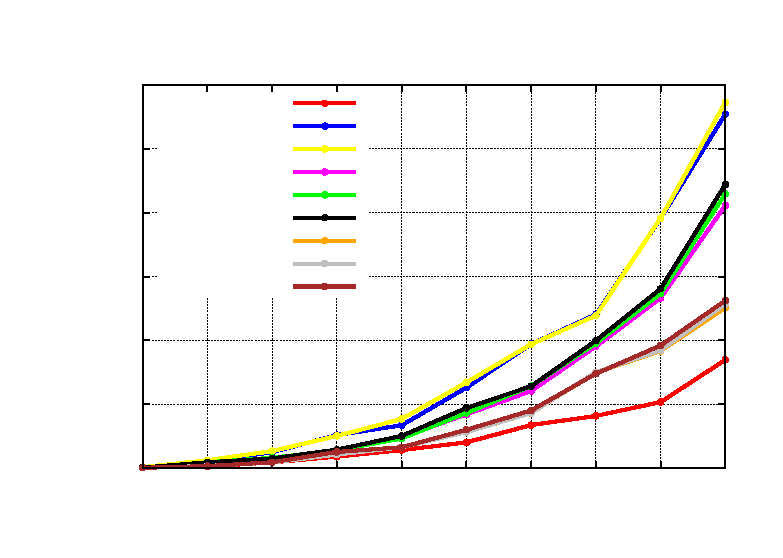
\includegraphics{points}}%
    \gplfronttext
  \end{picture}%
\endgroup

    \caption{Overview}
\end{figure}
\begin{figure}[!ht]
    \centering
    % GNUPLOT: LaTeX picture with Postscript
\begingroup
  \makeatletter
  \providecommand\color[2][]{%
    \GenericError{(gnuplot) \space\space\space\@spaces}{%
      Package color not loaded in conjunction with
      terminal option `colourtext'%
    }{See the gnuplot documentation for explanation.%
    }{Either use 'blacktext' in gnuplot or load the package
      color.sty in LaTeX.}%
    \renewcommand\color[2][]{}%
  }%
  \providecommand\includegraphics[2][]{%
    \GenericError{(gnuplot) \space\space\space\@spaces}{%
      Package graphicx or graphics not loaded%
    }{See the gnuplot documentation for explanation.%
    }{The gnuplot epslatex terminal needs graphicx.sty or graphics.sty.}%
    \renewcommand\includegraphics[2][]{}%
  }%
  \providecommand\rotatebox[2]{#2}%
  \@ifundefined{ifGPcolor}{%
    \newif\ifGPcolor
    \GPcolorfalse
  }{}%
  \@ifundefined{ifGPblacktext}{%
    \newif\ifGPblacktext
    \GPblacktexttrue
  }{}%
  % define a \g@addto@macro without @ in the name:
  \let\gplgaddtomacro\g@addto@macro
  % define empty templates for all commands taking text:
  \gdef\gplbacktext{}%
  \gdef\gplfronttext{}%
  \makeatother
  \ifGPblacktext
    % no textcolor at all
    \def\colorrgb#1{}%
    \def\colorgray#1{}%
  \else
    % gray or color?
    \ifGPcolor
      \def\colorrgb#1{\color[rgb]{#1}}%
      \def\colorgray#1{\color[gray]{#1}}%
      \expandafter\def\csname LTw\endcsname{\color{white}}%
      \expandafter\def\csname LTb\endcsname{\color{black}}%
      \expandafter\def\csname LTa\endcsname{\color{black}}%
      \expandafter\def\csname LT0\endcsname{\color[rgb]{1,0,0}}%
      \expandafter\def\csname LT1\endcsname{\color[rgb]{0,1,0}}%
      \expandafter\def\csname LT2\endcsname{\color[rgb]{0,0,1}}%
      \expandafter\def\csname LT3\endcsname{\color[rgb]{1,0,1}}%
      \expandafter\def\csname LT4\endcsname{\color[rgb]{0,1,1}}%
      \expandafter\def\csname LT5\endcsname{\color[rgb]{1,1,0}}%
      \expandafter\def\csname LT6\endcsname{\color[rgb]{0,0,0}}%
      \expandafter\def\csname LT7\endcsname{\color[rgb]{1,0.3,0}}%
      \expandafter\def\csname LT8\endcsname{\color[rgb]{0.5,0.5,0.5}}%
    \else
      % gray
      \def\colorrgb#1{\color{black}}%
      \def\colorgray#1{\color[gray]{#1}}%
      \expandafter\def\csname LTw\endcsname{\color{white}}%
      \expandafter\def\csname LTb\endcsname{\color{black}}%
      \expandafter\def\csname LTa\endcsname{\color{black}}%
      \expandafter\def\csname LT0\endcsname{\color{black}}%
      \expandafter\def\csname LT1\endcsname{\color{black}}%
      \expandafter\def\csname LT2\endcsname{\color{black}}%
      \expandafter\def\csname LT3\endcsname{\color{black}}%
      \expandafter\def\csname LT4\endcsname{\color{black}}%
      \expandafter\def\csname LT5\endcsname{\color{black}}%
      \expandafter\def\csname LT6\endcsname{\color{black}}%
      \expandafter\def\csname LT7\endcsname{\color{black}}%
      \expandafter\def\csname LT8\endcsname{\color{black}}%
    \fi
  \fi
  \setlength{\unitlength}{0.0500bp}%
  \begin{picture}(7200.00,5040.00)%
    \gplgaddtomacro\gplbacktext{%
      \csname LTb\endcsname%
      \put(1078,704){\makebox(0,0)[r]{\strut{} 0}}%
      \csname LTb\endcsname%
      \put(1078,1317){\makebox(0,0)[r]{\strut{} 200}}%
      \csname LTb\endcsname%
      \put(1078,1929){\makebox(0,0)[r]{\strut{} 400}}%
      \csname LTb\endcsname%
      \put(1078,2542){\makebox(0,0)[r]{\strut{} 600}}%
      \csname LTb\endcsname%
      \put(1078,3154){\makebox(0,0)[r]{\strut{} 800}}%
      \csname LTb\endcsname%
      \put(1078,3767){\makebox(0,0)[r]{\strut{} 1000}}%
      \csname LTb\endcsname%
      \put(1078,4379){\makebox(0,0)[r]{\strut{} 1200}}%
      \csname LTb\endcsname%
      \put(1210,484){\makebox(0,0){\strut{} 5}}%
      \csname LTb\endcsname%
      \put(1831,484){\makebox(0,0){\strut{} 10}}%
      \csname LTb\endcsname%
      \put(2453,484){\makebox(0,0){\strut{} 15}}%
      \csname LTb\endcsname%
      \put(3074,484){\makebox(0,0){\strut{} 20}}%
      \csname LTb\endcsname%
      \put(3696,484){\makebox(0,0){\strut{} 25}}%
      \csname LTb\endcsname%
      \put(4317,484){\makebox(0,0){\strut{} 30}}%
      \csname LTb\endcsname%
      \put(4939,484){\makebox(0,0){\strut{} 35}}%
      \csname LTb\endcsname%
      \put(5560,484){\makebox(0,0){\strut{} 40}}%
      \csname LTb\endcsname%
      \put(6182,484){\makebox(0,0){\strut{} 45}}%
      \csname LTb\endcsname%
      \put(6803,484){\makebox(0,0){\strut{} 50}}%
      \put(176,2541){\rotatebox{-270}{\makebox(0,0){\strut{}Processing time (s)}}}%
      \put(4006,154){\makebox(0,0){\strut{}Points to place}}%
      \put(4006,4709){\makebox(0,0){\strut{}Varying amount of points to place}}%
    }%
    \gplgaddtomacro\gplfronttext{%
      \csname LTb\endcsname%
      \put(2530,4206){\makebox(0,0)[r]{\strut{}1 n 2 ppn}}%
      \csname LTb\endcsname%
      \put(2530,3986){\makebox(0,0)[r]{\strut{}2 n 1 ppn}}%
    }%
    \gplbacktext
    \put(0,0){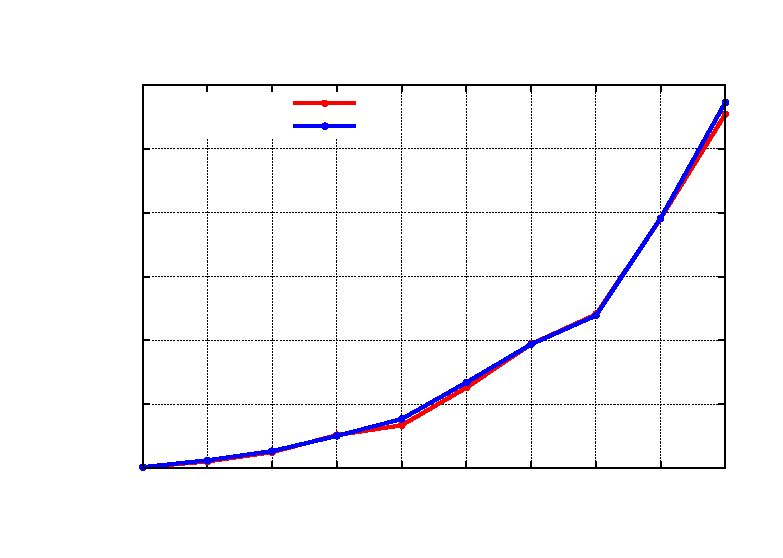
\includegraphics{points2}}%
    \gplfronttext
  \end{picture}%
\endgroup

    \caption{2 processors}
\end{figure}
\begin{figure}[!ht]
    \centering
    % GNUPLOT: LaTeX picture with Postscript
\begingroup
  \makeatletter
  \providecommand\color[2][]{%
    \GenericError{(gnuplot) \space\space\space\@spaces}{%
      Package color not loaded in conjunction with
      terminal option `colourtext'%
    }{See the gnuplot documentation for explanation.%
    }{Either use 'blacktext' in gnuplot or load the package
      color.sty in LaTeX.}%
    \renewcommand\color[2][]{}%
  }%
  \providecommand\includegraphics[2][]{%
    \GenericError{(gnuplot) \space\space\space\@spaces}{%
      Package graphicx or graphics not loaded%
    }{See the gnuplot documentation for explanation.%
    }{The gnuplot epslatex terminal needs graphicx.sty or graphics.sty.}%
    \renewcommand\includegraphics[2][]{}%
  }%
  \providecommand\rotatebox[2]{#2}%
  \@ifundefined{ifGPcolor}{%
    \newif\ifGPcolor
    \GPcolorfalse
  }{}%
  \@ifundefined{ifGPblacktext}{%
    \newif\ifGPblacktext
    \GPblacktexttrue
  }{}%
  % define a \g@addto@macro without @ in the name:
  \let\gplgaddtomacro\g@addto@macro
  % define empty templates for all commands taking text:
  \gdef\gplbacktext{}%
  \gdef\gplfronttext{}%
  \makeatother
  \ifGPblacktext
    % no textcolor at all
    \def\colorrgb#1{}%
    \def\colorgray#1{}%
  \else
    % gray or color?
    \ifGPcolor
      \def\colorrgb#1{\color[rgb]{#1}}%
      \def\colorgray#1{\color[gray]{#1}}%
      \expandafter\def\csname LTw\endcsname{\color{white}}%
      \expandafter\def\csname LTb\endcsname{\color{black}}%
      \expandafter\def\csname LTa\endcsname{\color{black}}%
      \expandafter\def\csname LT0\endcsname{\color[rgb]{1,0,0}}%
      \expandafter\def\csname LT1\endcsname{\color[rgb]{0,1,0}}%
      \expandafter\def\csname LT2\endcsname{\color[rgb]{0,0,1}}%
      \expandafter\def\csname LT3\endcsname{\color[rgb]{1,0,1}}%
      \expandafter\def\csname LT4\endcsname{\color[rgb]{0,1,1}}%
      \expandafter\def\csname LT5\endcsname{\color[rgb]{1,1,0}}%
      \expandafter\def\csname LT6\endcsname{\color[rgb]{0,0,0}}%
      \expandafter\def\csname LT7\endcsname{\color[rgb]{1,0.3,0}}%
      \expandafter\def\csname LT8\endcsname{\color[rgb]{0.5,0.5,0.5}}%
    \else
      % gray
      \def\colorrgb#1{\color{black}}%
      \def\colorgray#1{\color[gray]{#1}}%
      \expandafter\def\csname LTw\endcsname{\color{white}}%
      \expandafter\def\csname LTb\endcsname{\color{black}}%
      \expandafter\def\csname LTa\endcsname{\color{black}}%
      \expandafter\def\csname LT0\endcsname{\color{black}}%
      \expandafter\def\csname LT1\endcsname{\color{black}}%
      \expandafter\def\csname LT2\endcsname{\color{black}}%
      \expandafter\def\csname LT3\endcsname{\color{black}}%
      \expandafter\def\csname LT4\endcsname{\color{black}}%
      \expandafter\def\csname LT5\endcsname{\color{black}}%
      \expandafter\def\csname LT6\endcsname{\color{black}}%
      \expandafter\def\csname LT7\endcsname{\color{black}}%
      \expandafter\def\csname LT8\endcsname{\color{black}}%
    \fi
  \fi
  \setlength{\unitlength}{0.0500bp}%
  \begin{picture}(7200.00,5040.00)%
    \gplgaddtomacro\gplbacktext{%
      \csname LTb\endcsname%
      \put(946,704){\makebox(0,0)[r]{\strut{} 0}}%
      \csname LTb\endcsname%
      \put(946,1112){\makebox(0,0)[r]{\strut{} 100}}%
      \csname LTb\endcsname%
      \put(946,1521){\makebox(0,0)[r]{\strut{} 200}}%
      \csname LTb\endcsname%
      \put(946,1929){\makebox(0,0)[r]{\strut{} 300}}%
      \csname LTb\endcsname%
      \put(946,2337){\makebox(0,0)[r]{\strut{} 400}}%
      \csname LTb\endcsname%
      \put(946,2746){\makebox(0,0)[r]{\strut{} 500}}%
      \csname LTb\endcsname%
      \put(946,3154){\makebox(0,0)[r]{\strut{} 600}}%
      \csname LTb\endcsname%
      \put(946,3562){\makebox(0,0)[r]{\strut{} 700}}%
      \csname LTb\endcsname%
      \put(946,3971){\makebox(0,0)[r]{\strut{} 800}}%
      \csname LTb\endcsname%
      \put(946,4379){\makebox(0,0)[r]{\strut{} 900}}%
      \csname LTb\endcsname%
      \put(1078,484){\makebox(0,0){\strut{} 5}}%
      \csname LTb\endcsname%
      \put(1714,484){\makebox(0,0){\strut{} 10}}%
      \csname LTb\endcsname%
      \put(2350,484){\makebox(0,0){\strut{} 15}}%
      \csname LTb\endcsname%
      \put(2986,484){\makebox(0,0){\strut{} 20}}%
      \csname LTb\endcsname%
      \put(3622,484){\makebox(0,0){\strut{} 25}}%
      \csname LTb\endcsname%
      \put(4259,484){\makebox(0,0){\strut{} 30}}%
      \csname LTb\endcsname%
      \put(4895,484){\makebox(0,0){\strut{} 35}}%
      \csname LTb\endcsname%
      \put(5531,484){\makebox(0,0){\strut{} 40}}%
      \csname LTb\endcsname%
      \put(6167,484){\makebox(0,0){\strut{} 45}}%
      \csname LTb\endcsname%
      \put(6803,484){\makebox(0,0){\strut{} 50}}%
      \put(176,2541){\rotatebox{-270}{\makebox(0,0){\strut{}Processing time (s)}}}%
      \put(3940,154){\makebox(0,0){\strut{}Points to place}}%
      \put(3940,4709){\makebox(0,0){\strut{}Varying amount of points to place}}%
    }%
    \gplgaddtomacro\gplfronttext{%
      \csname LTb\endcsname%
      \put(2398,4206){\makebox(0,0)[r]{\strut{}1 n 4 ppn}}%
      \csname LTb\endcsname%
      \put(2398,3986){\makebox(0,0)[r]{\strut{}2 n 2 ppn}}%
      \csname LTb\endcsname%
      \put(2398,3766){\makebox(0,0)[r]{\strut{}4 n 1 ppn}}%
    }%
    \gplbacktext
    \put(0,0){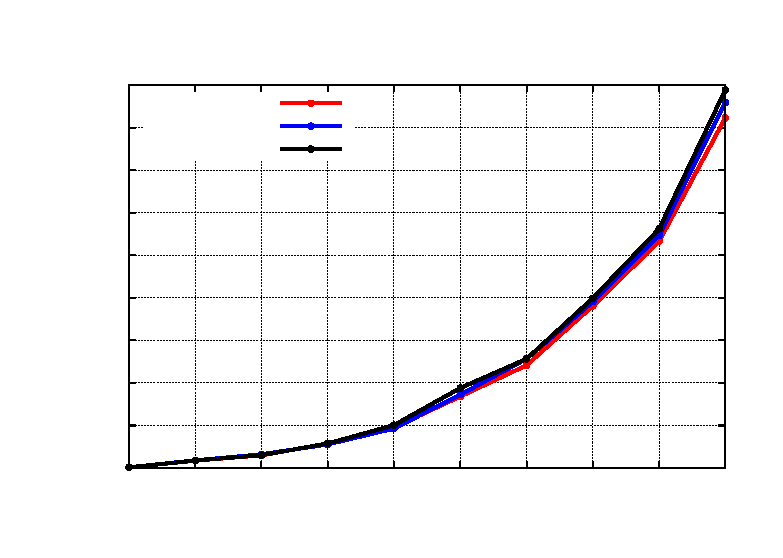
\includegraphics{points4}}%
    \gplfronttext
  \end{picture}%
\endgroup

    \caption{4 processors}
\end{figure}
\begin{figure}[!ht]
    \centering
    % GNUPLOT: LaTeX picture with Postscript
\begingroup
  \makeatletter
  \providecommand\color[2][]{%
    \GenericError{(gnuplot) \space\space\space\@spaces}{%
      Package color not loaded in conjunction with
      terminal option `colourtext'%
    }{See the gnuplot documentation for explanation.%
    }{Either use 'blacktext' in gnuplot or load the package
      color.sty in LaTeX.}%
    \renewcommand\color[2][]{}%
  }%
  \providecommand\includegraphics[2][]{%
    \GenericError{(gnuplot) \space\space\space\@spaces}{%
      Package graphicx or graphics not loaded%
    }{See the gnuplot documentation for explanation.%
    }{The gnuplot epslatex terminal needs graphicx.sty or graphics.sty.}%
    \renewcommand\includegraphics[2][]{}%
  }%
  \providecommand\rotatebox[2]{#2}%
  \@ifundefined{ifGPcolor}{%
    \newif\ifGPcolor
    \GPcolorfalse
  }{}%
  \@ifundefined{ifGPblacktext}{%
    \newif\ifGPblacktext
    \GPblacktexttrue
  }{}%
  % define a \g@addto@macro without @ in the name:
  \let\gplgaddtomacro\g@addto@macro
  % define empty templates for all commands taking text:
  \gdef\gplbacktext{}%
  \gdef\gplfronttext{}%
  \makeatother
  \ifGPblacktext
    % no textcolor at all
    \def\colorrgb#1{}%
    \def\colorgray#1{}%
  \else
    % gray or color?
    \ifGPcolor
      \def\colorrgb#1{\color[rgb]{#1}}%
      \def\colorgray#1{\color[gray]{#1}}%
      \expandafter\def\csname LTw\endcsname{\color{white}}%
      \expandafter\def\csname LTb\endcsname{\color{black}}%
      \expandafter\def\csname LTa\endcsname{\color{black}}%
      \expandafter\def\csname LT0\endcsname{\color[rgb]{1,0,0}}%
      \expandafter\def\csname LT1\endcsname{\color[rgb]{0,1,0}}%
      \expandafter\def\csname LT2\endcsname{\color[rgb]{0,0,1}}%
      \expandafter\def\csname LT3\endcsname{\color[rgb]{1,0,1}}%
      \expandafter\def\csname LT4\endcsname{\color[rgb]{0,1,1}}%
      \expandafter\def\csname LT5\endcsname{\color[rgb]{1,1,0}}%
      \expandafter\def\csname LT6\endcsname{\color[rgb]{0,0,0}}%
      \expandafter\def\csname LT7\endcsname{\color[rgb]{1,0.3,0}}%
      \expandafter\def\csname LT8\endcsname{\color[rgb]{0.5,0.5,0.5}}%
    \else
      % gray
      \def\colorrgb#1{\color{black}}%
      \def\colorgray#1{\color[gray]{#1}}%
      \expandafter\def\csname LTw\endcsname{\color{white}}%
      \expandafter\def\csname LTb\endcsname{\color{black}}%
      \expandafter\def\csname LTa\endcsname{\color{black}}%
      \expandafter\def\csname LT0\endcsname{\color{black}}%
      \expandafter\def\csname LT1\endcsname{\color{black}}%
      \expandafter\def\csname LT2\endcsname{\color{black}}%
      \expandafter\def\csname LT3\endcsname{\color{black}}%
      \expandafter\def\csname LT4\endcsname{\color{black}}%
      \expandafter\def\csname LT5\endcsname{\color{black}}%
      \expandafter\def\csname LT6\endcsname{\color{black}}%
      \expandafter\def\csname LT7\endcsname{\color{black}}%
      \expandafter\def\csname LT8\endcsname{\color{black}}%
    \fi
  \fi
  \setlength{\unitlength}{0.0500bp}%
  \begin{picture}(7200.00,5040.00)%
    \gplgaddtomacro\gplbacktext{%
      \csname LTb\endcsname%
      \put(946,704){\makebox(0,0)[r]{\strut{} 0}}%
      \csname LTb\endcsname%
      \put(946,1317){\makebox(0,0)[r]{\strut{} 100}}%
      \csname LTb\endcsname%
      \put(946,1929){\makebox(0,0)[r]{\strut{} 200}}%
      \csname LTb\endcsname%
      \put(946,2542){\makebox(0,0)[r]{\strut{} 300}}%
      \csname LTb\endcsname%
      \put(946,3154){\makebox(0,0)[r]{\strut{} 400}}%
      \csname LTb\endcsname%
      \put(946,3767){\makebox(0,0)[r]{\strut{} 500}}%
      \csname LTb\endcsname%
      \put(946,4379){\makebox(0,0)[r]{\strut{} 600}}%
      \csname LTb\endcsname%
      \put(1078,484){\makebox(0,0){\strut{} 5}}%
      \csname LTb\endcsname%
      \put(1714,484){\makebox(0,0){\strut{} 10}}%
      \csname LTb\endcsname%
      \put(2350,484){\makebox(0,0){\strut{} 15}}%
      \csname LTb\endcsname%
      \put(2986,484){\makebox(0,0){\strut{} 20}}%
      \csname LTb\endcsname%
      \put(3622,484){\makebox(0,0){\strut{} 25}}%
      \csname LTb\endcsname%
      \put(4259,484){\makebox(0,0){\strut{} 30}}%
      \csname LTb\endcsname%
      \put(4895,484){\makebox(0,0){\strut{} 35}}%
      \csname LTb\endcsname%
      \put(5531,484){\makebox(0,0){\strut{} 40}}%
      \csname LTb\endcsname%
      \put(6167,484){\makebox(0,0){\strut{} 45}}%
      \csname LTb\endcsname%
      \put(6803,484){\makebox(0,0){\strut{} 50}}%
      \put(176,2541){\rotatebox{-270}{\makebox(0,0){\strut{}Processing time (s)}}}%
      \put(3940,154){\makebox(0,0){\strut{}Points to place}}%
      \put(3940,4709){\makebox(0,0){\strut{}Varying amount of points to place}}%
    }%
    \gplgaddtomacro\gplfronttext{%
      \csname LTb\endcsname%
      \put(2398,4206){\makebox(0,0)[r]{\strut{}1 n 8 ppn}}%
      \csname LTb\endcsname%
      \put(2398,3986){\makebox(0,0)[r]{\strut{}2 n 4 ppn}}%
      \csname LTb\endcsname%
      \put(2398,3766){\makebox(0,0)[r]{\strut{}4 n 2 ppn}}%
    }%
    \gplbacktext
    \put(0,0){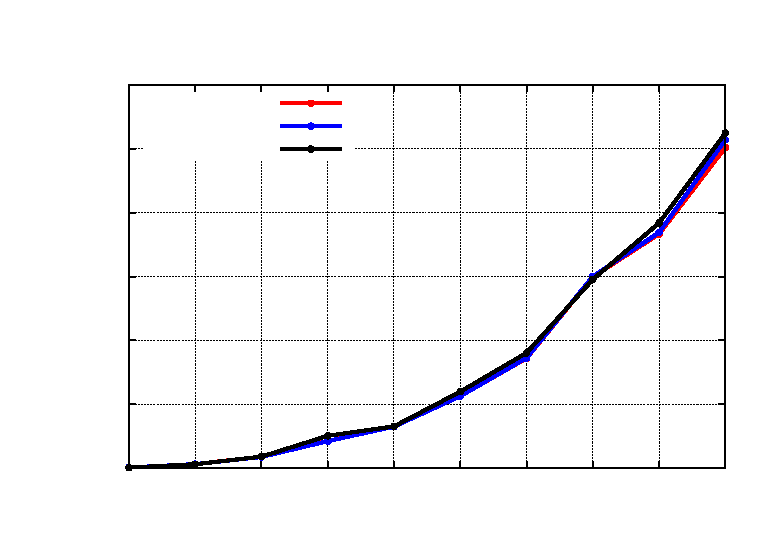
\includegraphics{points8}}%
    \gplfronttext
  \end{picture}%
\endgroup

    \caption{8 processors}
\end{figure} \\
Ook al is het in geen van de grafieken zeer duidelijk, toch kunnen we in elke grafiek zien dat het sneller is om het programma op zo weinig mogelijk verschillende machines te gebruiken. We zien ook dat het niet gedistribueerde programma redelijk wat sneller is. Dat is omdat de algoritmes toen nog niet waren geoptimaliseerd. In de testen hieronder zullen we grafieken geven waar ons gedistribueerd algoritme wel beter is. Het is logisch dat de executie op meerdere machines trager zou zijn dan deze op \'e\'en machien met evenveel cores, de communicatie duurt namelijk langer tussen machines heen dan in eenzelfde machine. Het feit dat we dit op de HPC, die infiniband gebruikt, mochten testen zorgt er voor dat we slechts weinig verschil zien.
\section{Wrappers}
Om slecht opspoorbare bugs en verrassingen tegen te gaan heb ik wrappers ge\"implementeerd rond de allocatie methoden en de free methode. Dit deed ik ook voor al mijn gebruikte MPI methodes. Voor de allocaties kijk ik gewoon of deze succesvol was, is dit niet zo dan print ik een foutmelding uit en stop ik het programma, bij de free zet ik telkens de pointer terug op NULL.\\
Voor MPI kijk ik of de operatie succesvol was, zoniet print ik een fout uit naar standard error.
\section{Testen}
Om het algoritme te verbeteren heb ik parameter per parameter (deze vind je terug in \verb|polygon.c| en \verb|genetic_algorithm.c|) proberen te optimaliseren. Ideaal zouden we natuurlijk alle mogelijkheden van parameters testen maar dit is tijdsgewijs niet mogelijk. Voor deze testen maakte ik gebruik van de voorbeeldinvoer en van een licht aangepaste versie hiervan. Deze aangepaste versie vermenigvuldigt gewoon elk punt van de voorbeeldinvoer met 100. Dit doen we om te zien hoe goed ons algoritme werkt op een veel grotere veelhoek. Op deze laatste heb ik niet getest indien expliciet vermeld. \\
Alle testen werden uitgevoerd met een willekeurige seed, dit omdat een vaste seed niet representatief is voor ons probleem. Om toch de effecten van de parameters te kunnen beoordelen voer ik de tests vijf keer uit en neem het gemiddelde van de vijf waarden.
De geschreven testen waren simpele bash scripts die gwn een parameter aanpassen in de bestand m.b.v. sed. Daarna voeren ze het bestand vijf keer uit en berekenen ze het gemiddelde van de fitness en de uitvoertijd m.b.v. bc. De tijd werd gemeten in C zelf m.b.v. \verb|clock()|.\\ Ik zal in de volgende puntjes tabellen gebruiken om de resultaten van mijn testen in weer te geven, rode rijen zijn rijen waarvoor de tijd en/of fitness in het oog springen.\par
\subsection{Populatiegrootte}
Mijn algoritme heeft een complexiteit van $i * (n * log(n))$ met $i$ het aantal iteraties en $n$ de grootte van de populatie. Voor de uitvoeringstijd te verbeteren willen we dus een zo klein mogelijke populatie gebruiken. \par
\begin{changemargin}{-1cm}{-1cm}
\begin{tabu}{r|l|l}
n&tijd (s)&fitness\\
\hline
5&1.333299&44.285213\\
10&1.316534&44.285213\\
15&1.335125&44.285213\\
20&1.408119&44.285213\\
25&1.317366&44.285213\\
30&1.339892&44.285213\\
35&1.343006&44.285213\\
40&1.324712&44.285213\\
45&1.328964&44.285213\\
50&1.302609&44.285213\\
\end{tabu}
\quad
\begin{tabu}{r|l|l}
n&tijd (s)&fitness\\
\hline
50&0.044704&44.186439\\
100&0.111102&44.224172\\
150&0.287113&44.267309\\
200&0.272872&44.258915\\
\rowfont{\color{red}}250&0.427653&44.282826\\
300&0.203128&44.247366\\
350&0.506790&44.267087\\
\rowfont{\color{red}}400&0.410105&44.284313\\
450&0.579759&44.255311\\
500&0.391176&44.238649\\
550&0.969413&44.271950\\
600&1.169380&44.283554\\
650&0.798042&44.277582\\
700&0.921339&44.269160\\
750&0.891495&44.252529\\
800&0.879678&44.277868\\
\rowfont{\color{red}}850&0.797560&44.291617\\
900&1.364649&44.288290\\
950&1.288533&44.285528\\
1000&1.358318&44.285213\\
\end{tabu}
\quad
\begin{tabu}{r|l|l}
n&tijd (s)&fitness\\
\hline
1000&1.275797&44.285213\\
1100&1.101109&44.287110\\
1200&2.513584&44.291963\\
1300&1.312317&44.275735\\
1400&2.216891&44.286630\\
1500&1.353093&44.277251\\
1600&2.408864&44.287080\\
1700&1.904357&44.298895\\
1800&2.702231&44.282092\\
1900&2.141803&44.280897\\
2000&2.185416&44.291120\\
\end{tabu}
\end{changemargin}
We zien dat we voor een grootte van 400 het beste resultaat verkrijgen.
\subsection{Mutatie kans}
Een grotere mutatiekans zorgt voor een betere variatie maar kan ook de tijd redelijk be\"invloeden omdat het steeds moeilijker wordt om een punt te muteren dat achteraf nog steeds in de veelhoek ligt.\par
\begin{centering}
\begin{tabu}{r|l|l}
kans&tijd (s)&fitness\\
\hline
5&1.252508&44.252762\\
10&1.644399&44.281032\\
15&1.161980&44.273699\\
20&0.866443&44.275032\\
25&1.108772&44.279561\\
\rowfont{\color{red}}30&0.803301&44.284923\\
35&1.349698&44.284897\\
\rowfont{\color{red}}40&1.857976&44.296939\\
45&1.014859&44.276939\\
50&1.592270&44.289612\\
\end{tabu}
\quad
\begin{tabu}{r|l|l}
kans&tijd (s)&fitness\\
\hline
55&1.729780&44.296507\\
60&1.124986&44.285807\\
65&1.020237&44.287012\\
70&1.138071&44.273711\\
75&1.534727&44.286223\\
\rowfont{\color{red}}80&1.967409&44.293574\\
85&1.921507&44.285273\\
90&1.406818&44.282038\\
\rowfont{\color{red}}95&1.317677&44.290561\\
100&2.207093&44.280363\\
\end{tabu}

\end{centering}\par
Hoewel hogere waarden accurater zijn geeft 30\% een goede balans tussen snelheid en accuraatheid.
\subsection{Aantal kinderen}
Aangezien het aantal kinderen een grote rol speelt in de complexiteit van ons algoritme, willen we het aantal kinderen zo laag mogelijk houden.\par
\begin{centering}
\begin{tabu}{r|l|l}
fractie&tijd (s)&fitness\\
\hline
0.1&0.590440&44.296455\\
\rowfont{\color{red}}0.2&0.534626&44.298437\\
\rowfont{\color{red}}0.3&0.597890&44.302311\\
0.33&0.835615&44.301361\\
0.4&1.716135&44.305364\\
0.5&1.174989&44.302785\\
\end{tabu}
\quad
\begin{tabu}{r|l|l}
fractie&tijd (s)&fitness\\
\hline
0.2&0.540695&44.301329\\
0.21&0.613173&44.300567\\
0.22&0.528419&44.300236\\
\rowfont{\color{red}}0.23&0.510684&44.302052\\
0.24&0.573765&44.300118\\
0.25&0.687835&44.298175\\
0.26&1.097019&44.300844\\
0.27&1.030754&44.302012\\
0.28&0.918490&44.302447\\
0.29&0.565139&44.296657\\
0.3&0.641136&44.297895\\
\end{tabu}

\end{centering}\par
De waarde $0.33$ werd beschouwd omdat dit in mijn tussentijdse versie werd gebruikt. We zien dat voor 0.23 de beste resultaten worden bereikt.
\subsection{Mutatiegrenzen}
Als we de mutatiegrenzen vergroten gaan we sneller aan een redelijke fitness komen en zal het algoritme snel genoeg stoppen. Met kleine grenzen kunnen we echter veel preciezer zijn en in sommige gevallen minder nutteloze stappen zetten waardoor kleinere grenzen zeker ook sneller kunnen zijn. Omdat ik vermoedde dat vaste grenzen een probleem zouden vormen op andere veelhoeken,  teste ik hier op zowel de kleine en grote veelhoek. A.h.v. de fitnesswaarde is duidelijk welke tabellen de grote en welke tabellen de kleine veelhoek voorstellen.\par
\begin{changemargin}{-1.4cm}{-1cm}
\begin{tabu}{r|l|l}
grens&tijd (s)&fitness\\
\hline
\rowfont{\color{red}}0.1&0.837893&44.303882\\
\rowfont{\color{red}}0.2&1.368992&44.305397\\
0.3&1.264244&44.298186\\
0.4&0.804467&44.299593\\
0.5&1.165631&44.298840\\
0.6&1.464119&44.298218\\
0.7&1.018262&44.291202\\
0.8&0.789543&44.280811\\
0.9&1.192347&44.289483\\
1.0&1.243368&44.268519\\
1.1&1.018943&44.281019\\
1.2&1.363694&44.285108\\
1.3&1.585455&44.283386\\
1.4&1.211326&44.277580\\
1.5&1.464460&44.278840\\
1.6&1.084871&44.265233\\
1.7&1.160951&44.264289\\
1.8&1.313925&44.276195\\
1.9&1.266772&44.274602\\
2.0&0.923208&44.266570\\
\end{tabu}
\,
\begin{tabu}{r|l|l}
grens&tijd (s)&fitness\\
\hline
0.1&10.631619&442.960956\\
0.2&7.699060&443.032693\\
0.3&6.542157&443.046798\\
0.4&4.374612&443.066404\\
0.5&1.533600&443.067654\\
0.6&5.159908&443.068675\\
0.7&1.789969&443.069246\\
0.8&2.275029&443.070129\\
0.9&1.789851&443.067485\\
1.0&1.983686&443.067817\\
1.1&1.472724&443.065066\\
1.2&2.507477&443.065850\\
1.3&1.735843&443.068938\\
1.4&2.012888&443.067546\\
1.5&1.350687&443.067512\\
1.6&1.547226&443.067241\\
1.7&1.732215&443.067082\\
1.8&1.490871&443.065617\\
1.9&1.618307&443.065145\\
2.0&1.205496&443.066685\\
\end{tabu}
\,
\begin{tabu}{r|l|l}
grens&tijd (s)&fitness\\
\hline
1&1.791540&443.068519\\
2&1.511818&443.067581\\
3&2.073624&443.067844\\
4&2.114675&443.068922\\
5&2.727197&443.067664\\
6&1.853344&443.066138\\
7&2.311777&443.067602\\
8&2.007532&443.068223\\
9&2.147488&443.067920\\
10&1.830200&443.068068\\
11&1.892601&443.067558\\
12&1.732955&443.069343\\
13&1.637722&443.066937\\
14&2.433165&443.067873\\
15&1.831892&443.068074\\
16&1.702581&443.066462\\
17&1.870442&443.068208\\
18&2.451833&443.066754\\
19&2.467672&443.067797\\
\rowfont{\color{red}}20&1.354229&443.066210\\
\end{tabu}

\end{changemargin}
We zien dus dat wanneer de grens 25 keer kleiner is dan de hoogte of breedte van de veelhoek (5 voor het kleine en 500 voor het grote voorbeeld), we een optimum bereiken. Hier koos ik dus om de mutatiegrenzen in te stellen in functie van de hoogte of breedte in plaats van ze een vaste waarde te geven.
\subsection{Fractie zeker overlevenden}
Door de fractie van de populatie die zeker overleeft te verhogen krijgen we minder variatie maar verzekeren we wel dat onze beste resultaten niet zomaar verdwijnen.\par
\begin{centering}
\begin{tabu}{r|l|l}
overlevenden&tijd (s)&fitness\\
\hline
0.05&1.053361&44.302225\\
\rowfont{\color{red}}0.10&0.976648&44.304833\\
0.15&0.910747&44.301297\\
0.20&0.834630&44.302787\\
0.25&0.911749&44.301497\\
0.30&0.854620&44.302442\\
0.35&0.920590&44.298910\\
0.40&0.848911&44.302714\\
\rowfont{\color{red}}0.45&0.801977&44.300442\\
0.50&0.956451&44.297539\\
0.55&0.579260&44.302316\\
0.60&1.068470&44.302443\\
0.65&1.109542&44.302372\\
0.70&0.944964&44.301569\\
0.75&1.401389&44.301480\\
\end{tabu}

\end{centering}\par
We zien dat 45\% iets minder accuraat is dan 10\% maar het is wel redelijk wat sneller, we maken dus gebruik van deze waarde.
\subsection{Aantal iteraties}
Ten slotte willen we nog het aantal iteraties dat we op eenzelfde waarde blijven hangen zo laag mogelijk krijgen.\par
\begin{centering}
\begin{tabu}{r|l|l}
iteraties&tijd (s)&fitness\\
\hline
\rowfont{\color{red}}100&0.175859&44.284295\\
200&0.215911&44.286928\\
300&0.353715&44.297873\\
400&0.299254&44.297000\\
500&0.325611&44.297000\\
600&0.488860&44.298113\\
700&0.474051&44.298694\\
800&0.493721&44.298694\\
\rowfont{\color{red}}900&0.643924&44.301477\\
1000&0.702387&44.301637\\
\end{tabu}

\end{centering}\par
We zien een zeer korte tijd voor slechts 100 iteraties maar dit gaat ten koste van de accuraatheid, we kiezen dus voor 900 aangezien dit ongeveer even accuraat is als 1000, maar wel sneller.
\subsection{Eindresultaat optimalisatie}
Voor we de parameters optimaliseerden kregen we waarden uit de bovenste tabel voor de kleine en de grote voorbeeldinvoer, na  optimalisatie deze in de onderste.\\
\begin{center}
    \begin{tabu}{r|l|l}
        invoer&uitvoertijd (s)&fitness\\\hline
        klein&0.745203&44.264378\\
        groot&1.528742&443.067074
    \end{tabu}
\end{center}
\begin{center}
    \begin{tabu}{r|l|l}
        invoer&uitvoertijd (s)&fitness\\\hline
        klein&0.392012&44.294878\\
        groot&0.528742&443.004874
    \end{tabu}
\end{center}
Voor het gedistribueerde algoritme vonden we op dezelfde manier:
\begin{center}
    \begin{tabu}{r|r|l|l}
        processen&invoer&uitvoertijd (s)&fitness\\\hline
        2&klein&0.398732&44.288367\\
        3&klein&0.464918&44.296163\\
        4&klein&0.508742&44.298040\\
        2&groot&0.982952&443.068167\\
        3&groot&1.068391&443.068759\\
        4&groot&1.278585&443.069555
    \end{tabu}
\end{center}
\begin{center}
    \begin{tabu}{r|r|l|l}
        processen&invoer&uitvoertijd (s)&fitness\\\hline
        2&klein&0.196203&44.301142\\
        3&klein&0.148199&44.303593\\
        4&klein&0.106849&44.303030\\
        2&groot&0.322740&443.027143\\
        3&groot&0.276021&443.031589\\
        4&groot&0.246178&443.034127
    \end{tabu}
\end{center}\par
We kunnen dus spreken van een fikse verbetering, zowel op \'e\'en core als meerdere is de snelheid voor het grote voorbeeld verdrievoudigd en voor de kleine is het verdubbeld. We zien ook dat de accuraatheid voor de kleine verbeterd is en die van de grootte iets achteruit is gegaan. Dit is omdat de mutatiegrenzen zijn aangepast naar dynamische waarden i.p.v. kleine vaste waarden (0.9 tijdens tussentijdse versie).
\subsection{Correctheidtesten}
Om te testen op memory leaks maakte ik gebruik van crtdbg op Windows. Eens ik ben begonnen met MPI heb ik geen geheugen meer gealloceerd dus het is niet erg dat ik dit niet goed kon testen op Windows. Om zekerheid te krijgen over mijn algoritme controleerde ik of de punten die uit het algoritme komen wel degelijk binnen de veelhoek lagen, ik heb hiervoor ook af en toe gebruik gemaakt van de visualisatie tool die werd meegeleverd.\\ Af en toe wordt er wel een punt in de aard van 0.000000 afgeprint, dit is normaal niet legaal volgens de opgave als we het standaardvoorbeeld gebruiken. Ik denk dat dit probleem echter ligt aan de print aangezien ik test of het punt niet op de hoogste of laagste y-waarde van mijn veelhoek ligt helemaal in het begin van de methode \verb|is_point_in_polygon|.
\end{document}